\documentclass{article}
\usepackage[utf8]{inputenc}
\usepackage[T1]{fontenc}
\usepackage[francais]{babel}
\usepackage{amsmath,amssymb}
\usepackage{fullpage}
\usepackage[pdftex]{graphicx}
\usepackage{xspace}
\usepackage{verbatim}
\usepackage{graphicx}
\usepackage{listings}
\usepackage[usenames,dvipsnames]{color}
\usepackage{url}
\usepackage{xcolor}


\title{Traitement image}
\author{Guidet Ulysse \\ Remy Lavainne}
\date{March 2019}

\begin{document}

\maketitle

\section{Filtrage Gaussien}

\begin{figure}[h]
 \begin{minipage}[b]{.46\linewidth}
  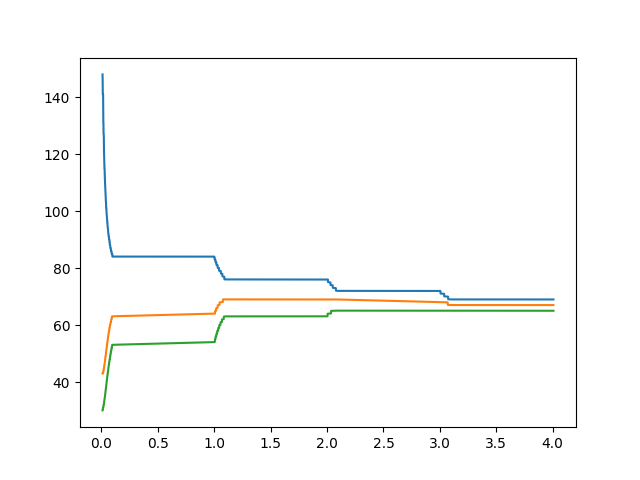
\includegraphics[scale=0.4]{form2bbbis.png}
\caption{Calcul PSNR :\textcolor{blue}{\rule{0.5cm}{0.03cm}} formes2b \textcolor{orange}{\rule{0.5cm}{0.03cm}}formes2bb30
\textcolor{green}{\rule{0.5cm}{0.03cm}} formes2bb60}
 \end{minipage} \hfill
 \begin{minipage}[b]{.46\linewidth}
  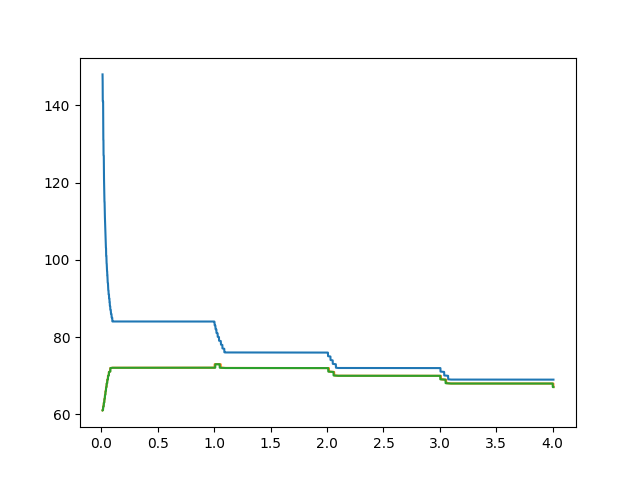
\includegraphics[scale=0.4]{form2p.png}
\caption{Calcul PSNR :\textcolor{blue}{\rule{0.5cm}{0.03cm}} formes2b \textcolor{orange}{\rule{0.5cm}{0.03cm}}formes2p2
\textcolor{green}{\rule{0.5cm}{0.03cm}} formes2p4}
 \end{minipage}
\end{figure}


\begin{figure}[h]
 \begin{minipage}[b]{.46\linewidth}
  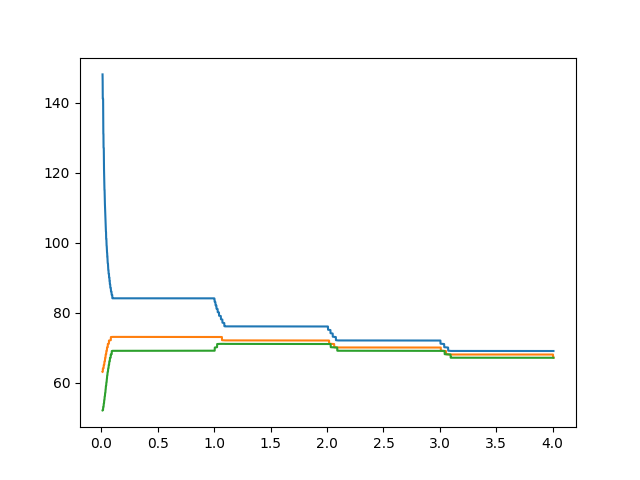
\includegraphics[scale=0.4]{form2s.png}
\caption{Calcul PSNR :\textcolor{blue}{\rule{0.5cm}{0.03cm}} formes2b \textcolor{orange}{\rule{0.5cm}{0.03cm}}formes2s30
\textcolor{green}{\rule{0.5cm}{0.03cm}} formes2s60}
 \end{minipage} \hfill
 \begin{minipage}[b]{.46\linewidth}
  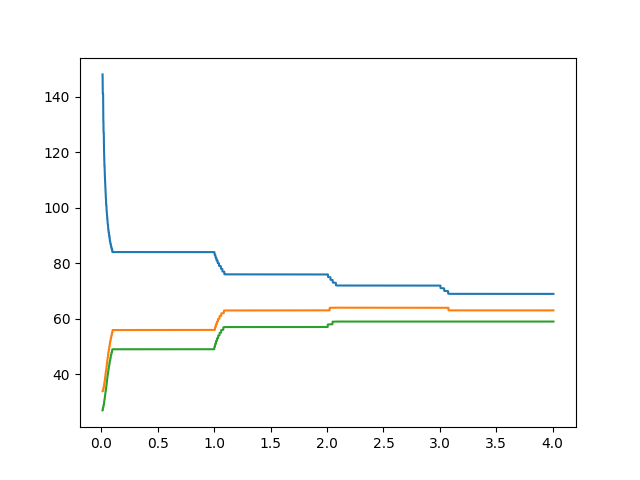
\includegraphics[scale=0.4]{form2sp.png}
\caption{\textcolor{blue}{\rule{0.5cm}{0.03cm}} formes2b \textcolor{orange}{\rule{0.5cm}{0.03cm}}formes2sp12
\textcolor{green}{\rule{0.5cm}{0.03cm}} formes2sp24}
 \end{minipage}
\end{figure}

On effectue un filtrage gaussien sur les différentes images bruitées et on calcule le PSNR entre les images obtenues et l'image formes2b.pgm. Les courbes représentent donc le PSNR obtenue en fonction de $\sigma$, le paramètre gaussien.

Pour une image de type poisson et speekle, le niveau de bruit n'influe pas le résultat filtrer. La valeur de sigma n'est pas non plus importante. On a quand même un meilleur résultat pour un $\sigma$ entre 0.1 et 2. Le filtrage gaussien est plus efficace pour ces types de bruit que pour les deux autres.
\newline
Pour les deux autres types de bruits, le niveau de bruit influe un peu plus que précédemment mais reste assez négligeable. Dans ces cas le filtre gaussien est plus efficace pour $\sigma \geq 1$
Dans tous les cas le PSNR entre l'image bruitée et filtrée décroit pour $\sigma \geq 3$.

\begin{figure}[h]
 \begin{minipage}[b]{.46\linewidth}
  \includegraphics[scale=0.4]{radio1Time.png}
  \caption{Temps radio1.pgm :\textcolor{blue}{\rule{0.5cm}{0.03cm}} filtrage Gaussien
\textcolor{orange}{\rule{0.5cm}{0.03cm}} convolution spatiale}
 \end{minipage} \hfill
 \begin{minipage}[b]{.46\linewidth}
  \includegraphics[scale=0.4]{forme2gTime.png}
\caption{Temps formes2g.pgm \textcolor{blue}{
\rule{0.5cm}{0.03cm}} filtrage Gaussien \textcolor{orange}{\rule{0.5cm}{0.03cm}}convolution spatiale}
 \end{minipage}
\end{figure}

\begin{figure}[h]
\includegraphics[scale=0.4]{radio1024.png}
\caption{Temps radio1024.pgm \textcolor{blue}{
\rule{0.5cm}{0.03cm}} filtrage Gaussien \textcolor{orange}{\rule{0.5cm}{0.03cm}}convolution spatiale}
\end{figure}

\section{Convolution spatiale}

On effectue une convolution spatiale séparable, avec comme parametre la taille du masque, qu'on regle en general en fonction de sigma.
On calcule l'EQM (ecart quadratique moyen) par rapport au filtre gaussien, la taille du masque est en proportion de sigma : N = W(\sigma) = a*\sigma :

\begin{tabular}{| a || b | c | d | e | f |}
    \hline
    a/sigma & 1 & 2 & 5 & 10 & 20 \\
    \hline
    1 & 663.821296 & 1867.795812 & 2953.494399 & 3338.244053 & 3514.698997 \\
    2 & 4.524510 & 28.070416 & 64.867759 & 82.120912 & 92.751862 \\
    3 & 0.019195 & 0.075842 & 0.225751 & 0.317130 & 0.658155 \\
    4 & 0.015186 & 0.018526 & 0.039034 & 0.055471 & 0.253320 \\
    5 & 0.015185 & 0.018501 & 0.039079 & 0.055575 & 0.251062 \\
    6 & 0.015185 & 0.018501 & 0.039081 & 0.055577 & 0.251043 \\
    \hline
 \end{tabular}


On remarque que pour a=1, l'ecart est tres grand entre les deux filtres. Ce parametrage n'est pas adapte.
On peut considerer que le filtre a convolution spatiale est proche du filtre gaussien a partir de a = 3.

\section{Détection de contour}

\subsection{Gradient}
On trouve le gradient par convolution avec une matrice de Sobel et on prend un seuil bas de 60 et un seuil haut de 100, pour l'image tangram on obtient les contours suivant :

\begin{figure}[h]
\includegraphics[scale=0.3]{contourTangram.png}

\end{figure}
\bigbreak
\bigbreak
\bigbreak
\bigbreak
\bigbreak
\bigbreak
\bigbreak
\bigbreak
\bigbreak
\bigbreak
\bigbreak
L'extraction de contour par gradient ne fonctionne pas du tout sur des images bruitées. Tous les contours ne sont pas détecter et l'image recu ne contient que des pixels nuls.

\subsection{Laplacien}

On calcule le laplacien par convolution avec un masque et par détection des valeurs nulles du laplacien on détecte les contours. Par cette recherche on obtient l'image suivante sur l'image tangram :
\begin{figure}[h]
\includegraphics[scale=0.4]{tangramlaplace.png}
\end{figure}

Les contours obtenus sont moins propre que par la méthode du gradient. Mais la recherche de contour par laplacien fonctionne à peu près sur les images bruitées :


\begin{figure}[h]
\includegraphics[scale=0.4]{contourbb.png}
\caption{Contour de formes2bb30.pgm}
\end{figure}

\begin{figure}[h]
\includegraphics[scale=0.4]{contour_s.png}
\caption{Contour de formes2s40.pgm}
\end{figure}
\begin{figure}[h]
\includegraphics[scale=0.4]{contour_sp.png}
\caption{Contour de formes2sp21.pgm}
\end{figure}
\begin{figure}[h]
\includegraphics[scale=0.4]{contour_p.png}
\caption{Contour de formes2p4.pgm}
\end{figure}
\end{document}
